\section{Wicklungsschema Übung 4}
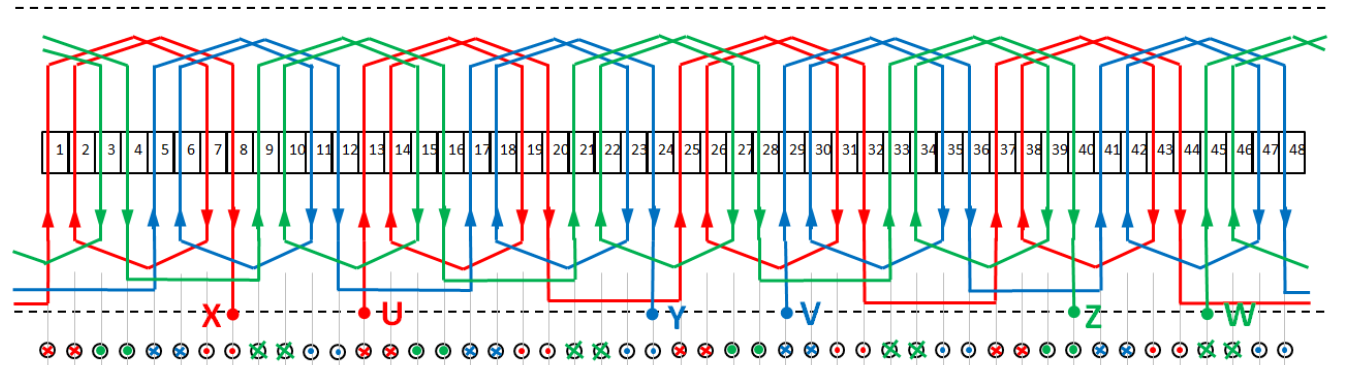
\includegraphics[scale = 0.5]{images/Wicklungsschema}
\subsection{Wichtige Formeln}
\begin{tabular}{|C{0.3\textwidth}|P{0.4\textwidth}|P{0.3\textwidth}}
	\hline
	\textbf{Drehzahl} & \[n = 60\cdot \dfrac{f}{p}\] & \vspace{0.05cm}n - Drehzahl [n] = $\dfrac{1}{min}$ \newline 
													   f - Frequenz \newline
													   p - Polpaarzahl 
\\ \hline
	\textbf{Nutzahl} & \[ N = 2p\cdot q\cdot m\] & 2p - Polzahl \newline 
												   q - Nutzahl pro Phasenband \newline
												   m - Strangzahl 
\\ \hline						 
\end{tabular}

\subsection{Beispiel}
\begin{minipage}[b]{0.4\linewidth}	
"\,8-polig "\quad$\widehat{=}$ \quad 2p = 8 \newline
N = 48 \newline
m = 3 \newline
q = 2 \newline \newline
$i_{L1} = Real\{\underline{I_{L1}}\} = 0.5\cdot I_0$ \newline \newline
$i_{L2} = Real\{\underline{I_{L2}}\} = 0.5\cdot I_0$ \newline \newline
$i_{L3} = Real\{\underline{I_{L3}}\} = -1.0\cdot I_0$ 
\newline \newline
	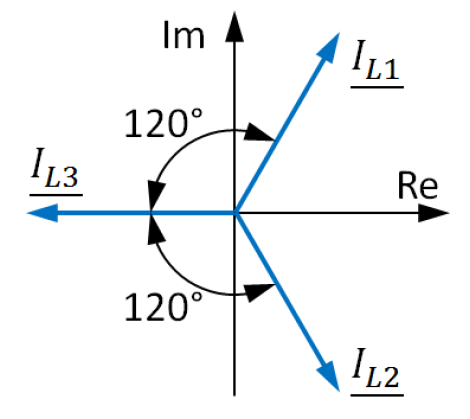
\includegraphics[scale = 0.4]{images/StromdreieckAGS}
\end{minipage}
\begin{minipage}[b]{0.4\linewidth}
	\raggedright
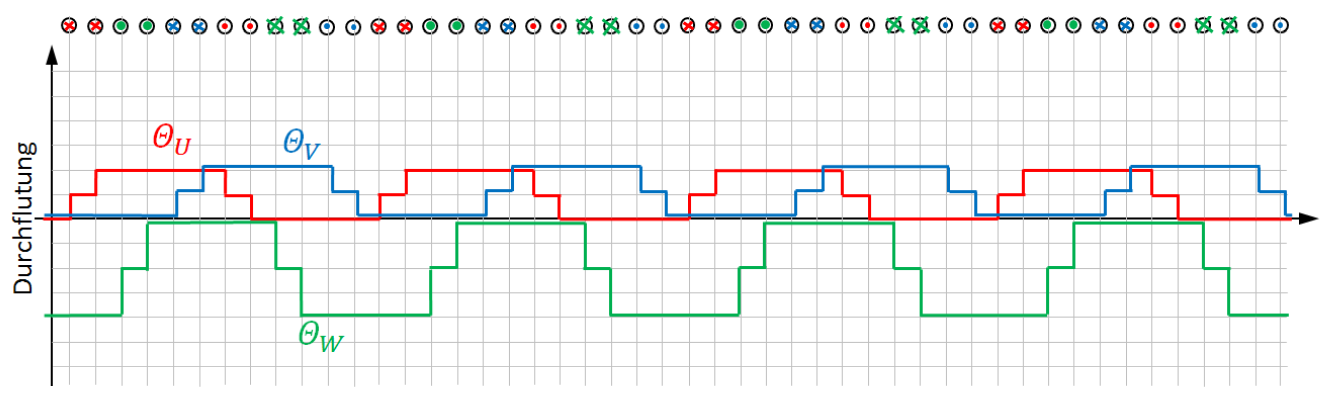
\includegraphics[scale = 0.35]{images/Durchflutung3} \newline
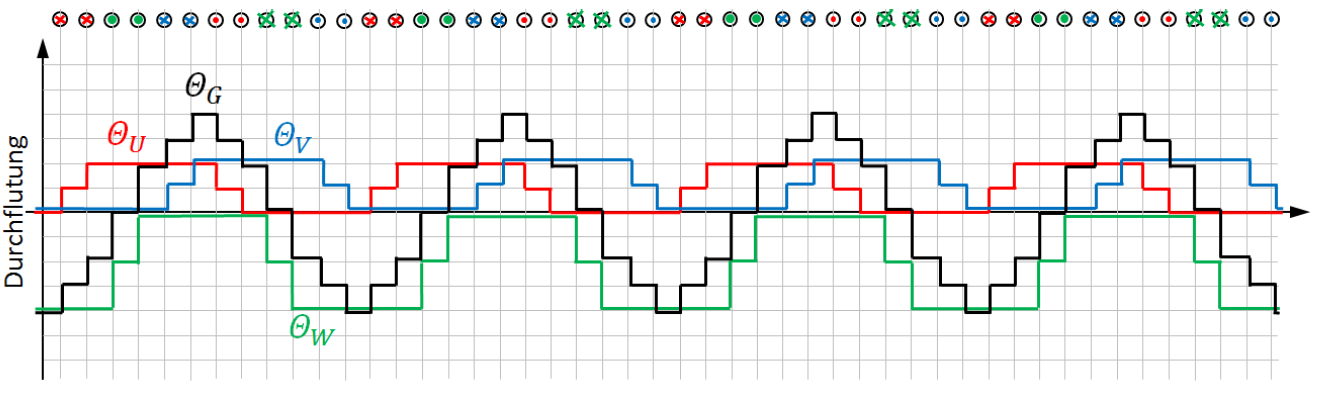
\includegraphics[scale = 0.35]{images/Durchflutung4} \newline

\end{minipage}
\clearpage